\clearpage
\section{Introduction}
\label{sec:Intro}
Agentic systems increasingly automate multi-step work in organizations. For each task of such a system, a software architect must decide whether predefined code or the model controls the progression of the task. Neither option is best for all tasks. This thesis develops and evaluates decision support for this choice. This chapter motivates the problem, derives the research gap and research questions, and outlines the research method together with the structure of the thesis.

\subsection{Motivation and Relevance}
\label{subsec:intro/motivation}
Organizations increasingly use artificial intelligence (AI) in their business activities. According to the AI Index 2025, the share of survey respondents reporting AI use in their organization rose from 55\% in 2023 to 78\% in 2024 \parencite{maslejArtificialIntelligenceIndex2025}. Agentic systems extend this use from single answers to multi-step work. They combine large language models (LLMs) with planning, tool use and memory to pursue a goal \parencite{dwivediAgenticAISystems2026,sapkotaAIAgentsVs2026}. Information systems (IS) research describes them as agentic information systems. Unlike reactive tools, they can make decisions on their own and act in unstructured environments \parencite{holldackAgenticInformationSystems2026}.

Organizations, however, realize the potential of AI and agentic systems only in part. In a 2026 McKinsey survey, eight in ten respondents reported that AI had improved their own productivity. Yet only 37\% reported that AI had contributed to the earnings before interest and taxes of their organization, about the same share as one year earlier \parencite{tinkoffStateAI2026}. The scaling of agentic systems is concentrated in large organizations. Among respondents from organizations with annual revenues above USD~1~billion, 40\% reported scaling such systems, up from 27\% one year earlier. Among smaller organizations, this share remained at 22\% \parencite{tinkoffStateAI2026}.

Two problems limit the use of agentic systems in particular: cost and reliability. In the same survey, about one in five respondents reported that AI-related operating costs, including token costs, had constrained the use of AI in their organization \parencite{tinkoffStateAI2026}. For agentic software development and complex reasoning tasks, the number of tokens has grown faster than the price per token has fallen \parencite{tinkoffStateAI2026}. \textcite{panMeasuringAgentsProduction2025} surveyed practitioners on 86 deployed agentic systems and conducted 20 case studies. Reliability was the top development challenge. Organizations often restricted early deployments to internal users to manage unresolved reliability, safety and security risks.

Both problems depend on how a system is designed. Practitioners currently address reliability through system-level design. Most deployed systems used simple and controllable designs: 68\% executed at most ten steps before a human intervened \parencite{panMeasuringAgentsProduction2025}. According to McKinsey, the organizations that move fastest treat operating costs as a design constraint \parencite{tinkoffStateAI2026}. A central part of this design is orchestration. It manages the control flow between model calls and tools according to predefined or adaptive execution policies \parencite{sapkotaLangChainVsLangGraph2025}. A key orchestration question is therefore how much control the model receives.

An agentic email-response process shows that a software architect must answer this question for each task. The process for example can be split into four tasks: triage, context gathering, draft composition and draft verification. Triage can apply written rules to each incoming email. Context gathering may need to decide during execution which source to search next. Two alternatives exist for each task. In an LLM workflow, code defines the possible execution paths, and the model performs bounded steps within them. In an agent, the model selects the next action and decides when the task is complete (Section~\ref{subsec:theory/workflows-agents}). This thesis calls these two alternatives orchestration paradigms.

The orchestration paradigm directly affects cost and reliability. Code-defined paths make execution predictable and consistent. Model control allows adaptation to new observations, but it raises cost and can compound errors \parencite{schluntzBuildingEffectiveAI2024}. The choice thus shifts the balance between task success, token cost, predictability and failure behavior.

Progress in models and implementations shifts these trade-offs but does not remove the choice. WorkBench is a benchmark of workplace tasks such as sending emails and scheduling meetings \parencite{stylesWorkBenchBenchmarkDataset2024}. In 2024, the best agent completed 43\% of its tasks. On a corrected version with native tool calls, the best agent completed 97.7\% in 2026, and harmful side effects fell from 26\% to 1.9\% of the tasks \parencite{stylesWorkBenchRevisitedWorkplace2026}. The same study found that the strongest models still made basic mistakes that occasionally caused irreversible harm, and that their costs stayed stable. In production, newer models do not guarantee better performance of an existing agentic system \parencite{panMeasuringAgentsProduction2025}. Cost and failure behavior therefore remain part of the choice.

Studies of agent designs show that no single design performs best. AgentArch compared 18 agent configurations on two enterprise use cases, and the best configuration differed between models and use cases \parencite{bogavelliAgentArchComprehensiveBenchmark2025}. \textcite{kimScienceScalingAgent2025} compared single agents with four multi-agent designs. Relative to a single agent, the performance change ranged from $+80.8$\% to $-70.0$\%, depending on the task structure. A preliminary test with three more capable models on one benchmark largely confirmed these patterns. Good performance thus depends on the fit between task, model and design.

This thesis uses the term agentic workplace automation for the automation of workplace and enterprise tasks with agentic systems. In this setting, the choice of an orchestration paradigm recurs for each task of each system. Drawing on projects in several organizations, \textcite{bandaraPracticalGuideAgentic2026} report that engineering teams often lack clear guidance on how to put agentic systems into operation. Software architects therefore need traceable decision support that links task characteristics to the control over task progression. 

\subsection{Problem}
\label{subsec:intro/problem}
The problem addressed in this thesis is how software architects can choose and justify an LLM workflow or an agent for a single task in agentic workplace automation. The choice is difficult because the qualities of the two orchestration paradigms compete. Higher task success can come at the price of more token cost or less predictability. The choice belongs to the class of architecture decisions that resolve trade-offs between quality attributes \parencite{falessiDecisionmakingTechniquesSoftware2011}. Decision support in information systems research has long focused on such semi-structured decisions \parencite{spragueFrameworkDevelopmentDecision1980}. Evidence can inform the comparison of the two orchestration paradigms. The weight of each quality, however, depends on the deployment and requires the judgment of the software architect.
 
Practitioner guidance offers a first heuristic. It recommends LLM workflows for well-defined tasks. Agents are recommended for open-ended problems  \parencite{schluntzBuildingEffectiveAI2024}. This guidance draws on experience of development teams. It names criteria but offers no procedure to assess them for a concrete task. Nor does it explain how to weigh competing priorities or how to justify the result.
 
Direct comparisons of the two orchestration paradigms point in opposite directions. In constraint-intensive travel planning, a code-controlled LLM workflow reached a higher pass rate than agent baselines \parencite{qiuBlueprintFirstModel2025}. In simulated procedural dialogues, model-controlled execution of a procedure given in the prompt reached higher judged task success than a code-controlled orchestration graph, but used more tokens \parencite{dennisInContextPromptingObsoletes2026}. Its authors conclude that stronger models make external orchestration unnecessary for such dialogues. Both studies concern tasks that follow a defined procedure, yet they favor opposite orchestration paradigms under their specific models and implementations. Neither provides a procedure for selecting an orchestration paradigm across workplace tasks.
 
Further research covers neighboring parts of the decision (Section~\ref{subsec:theory/related-work}). The studies of agent designs cited above do not compare code-controlled with model-controlled task progression \parencite{bogavelliAgentArchComprehensiveBenchmark2025,kimScienceScalingAgent2025}. Workplace benchmarks such as WorkBench and TheAgentCompany provide realistic tasks and outcome checks \parencite{stylesWorkBenchBenchmarkDataset2024,xuTheAgentCompanyBenchmarkingLLM2025}. Their original evaluations, however, test agents without a paired LLM workflow. A catalogue of agent design patterns offers qualitative selection guidance without paired execution evidence \parencite{liuAgentDesignPattern2025}. Routing approaches select or compose a reasoning or coordination strategy for each incoming request \parencite{gaoSingleagentMultiagentSystems2025,suDifficultyAwareAgenticOrchestration2025,zhouSelectthenSolveParadigmRouting2026}. They work at run time with components that are already implemented. A software architect, in contrast, decides before implementation and must justify the choice against the constraints and priorities of the deployment.
 
The research gap lies in connecting these parts. No reviewed approach lets software architects combine task characteristics, comparative execution evidence, constraints and priorities in one framework. Such a framework is needed to choose between an LLM workflow and an agent before implementation. Closing this gap requires two kinds of knowledge. The first is comparative evidence on how both orchestration paradigms perform across workplace tasks. The second is design knowledge on how to turn this evidence into justified recommendations that state the conditions of their implementation.

\subsection{Scope and Research Question}
\label{subsec:intro/scope}
This thesis develops and evaluates the Task-Level Architecture Decision Framework (TADF). Before implementation, TADF supports software architects in choosing an orchestration paradigm for single tasks in agentic systems for workplace automation. The software architect describes the task and states constraints and priorities. TADF then recommends an LLM workflow or an agent and explains the basis of this recommendation. It also provides implementation guidance, including the conditions on which the recommendation depends. Figure~\ref{fig:tadf-scope} summarizes this purpose.
 
\begin{figure}[htbp]
\centering
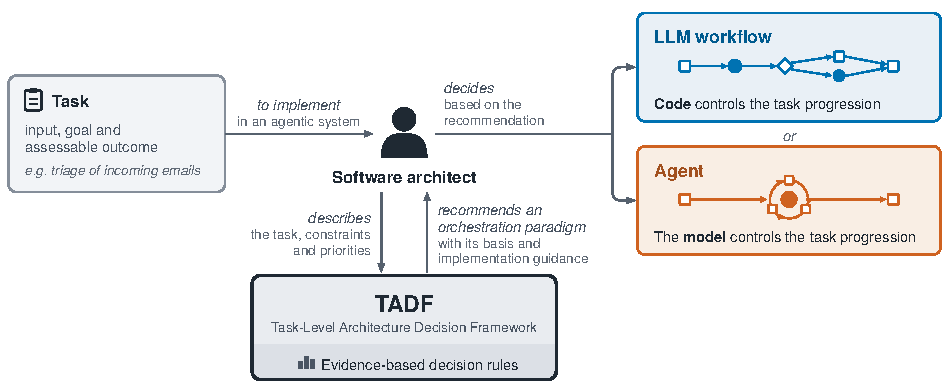
\includegraphics[width=\linewidth]{Figures/fig_tadf_scope (1).pdf}
\caption{Scope, functionality and context of the TADF.}
\label{fig:tadf-scope}
\end{figure}
 
The decision unit is a task: a bounded unit of work with an identifiable input, a coherent goal and an assessable outcome (Section~\ref{subsubsec:theory/task}). Before the comparison, TADF checks whether the task needs an LLM at all and whether it should be simplified or split into smaller tasks. This gives TADF four possible outcomes: deterministic implementation, decomposition, LLM workflow or agent. The coordination between tasks, the composition of several agents, the selection of an LLM and the operation of the deployed system lie outside its scope. The comparative evidence covers eight task archetypes, three OpenAI models and the implementations built for this thesis. TADF addresses the suitability of a model through implementation guidance, not through a model-selection procedure.
 
The research question is: (RQ) How can a task-level architecture decision framework be designed to support software architects in selecting between LLM workflows and agents for agentic workplace automation? Three sub-questions structure the answer: (SQ1) How do LLM workflows and agents compare in terms of task-relevant performance metrics across workplace tasks? (SQ2) Which task characteristics and execution conditions are associated with performance differences between LLM workflows and agents? (SQ3) How relevant is the distinction between LLM workflows and agents to architecture decisions in practice, and to what extent can the proposed framework support software architects in making these decisions? The research examines one hypothesis: A task-level architecture decision framework based on task characteristics provides consistent and practically useful recommendations for selecting between LLM workflows and agents in agentic workplace automation. This hypothesis is a design proposition, not a statistical hypothesis.
 
In design science research (DSR), the purpose of an artifact defines the goals that the artifact must meet \parencite{gregorPositioningPresentingDesign2013}. Section~\ref{subsec:TADF/objectives} derives eight design objectives from the purpose of TADF. They cover the decision core, decision quality and use and deployment. Consistency means that the same task characteristics, constraints and priorities lead to the same recommendation (O4). Practical usefulness has two parts. First, software architects find the recommendations relevant and can apply them with bounded effort (O2, O6, O7). Second, following the recommendations improves the trade-off between task success and token cost compared with using one orchestration paradigm for all tasks (O5). The first part concerns perceived usefulness, the second measured decision quality.
 
The thesis contributes to practice and to knowledge. For practice, TADF is a documented decision framework. It is delivered as a reusable set of instructions and reference documents for an LLM assistant. For knowledge, the thesis provides comparative evidence on both orchestration paradigms, based on a task taxonomy and paired implementations. The decision method of TADF and three design principles add design knowledge for decision support of this kind. Because practice currently addresses the problem with heuristics, the thesis aims at an improvement in the sense of \textcite{gregorPositioningPresentingDesign2013}: a better solution for a known problem.

\subsection{Research Method}
\label{subsec:intro/method}
The research question asks how an artifact should be designed. This thesis therefore follows DSR, in which knowledge about a problem and its solution is gained by building and applying an artifact \parencite{hevnerDesignScienceInformation2004}. A purely empirical comparison of the two orchestration paradigms could answer SQ1 and SQ2, but not the research question. A decision procedure must first be built, applied and revised before its value can be judged. In addition, DSR requires that the utility, quality and efficacy of an artifact be demonstrated through evaluation \parencite{hevnerDesignScienceInformation2004}. TADF is the artifact of this thesis. It is a framework that was first instantiated as a spreadsheet, the Decision Sheet, and later as the TADF skill framework. The paired implementations of both orchestration paradigms are not part of TADF, they provide its evidence.
 
The research follows the six activities of the design science research methodology (DSRM): problem identification and motivation, objectives of a solution, design and development, demonstration, evaluation and communication \parencite{article}. The entry point is problem-centered. The activities ran in iterations: results of the experiments and of each evaluation episode led to revisions of TADF. Such formative evaluation can be reported as part of the development \parencite{gregorPositioningPresentingDesign2013}. The demonstration is reported after the evaluation because it uses the version of TADF that resulted from both evaluation episodes. The three design principles were abstracted from these revisions and the evidence behind them, using the schema of \textcite{australiannationaluniversityaustraliaResearchPerspectivesAnatomy2020} (Section~\ref{subsec:discussion/contribution}).
 
In the three-cycle view of \textcite{hevnerThreeCycleView2007}, the iterative revisions form the design cycle. The rigor cycle and the relevance cycle link it to its context. The rigor cycle drew on a targeted literature review. It aimed to identify the concepts, theories and studies that the design of TADF requires, not to map the field completely. Keyword searches in Google Scholar, ScienceDirect and arXiv combined two groups of terms. The first described the systems, such as LLM workflow, agent, agentic workflow and multi-agent system. The second described the decision, such as orchestration, architecture decision and decision support. Backward snowballing from the included studies added further sources \parencite{wohlinGuidelinesSnowballingSystematic2014}. The searches were last updated in September 2026. Preprints were included because research on agentic systems moves faster than journal publication, and the bibliography records the version that was read. Documentation from AI providers and framework developers served only for definitions and practitioner guidance (Chapter~\ref{sec:theory}). In return, the comparative evidence and the design principles add to this knowledge base (Chapter~\ref{sec:discussion}). In the relevance cycle, reported practice motivated the problem. Practitioners assessed TADF once its initial version existed, and the demonstration applied the revised TADF to an external scenario. A field test in an organization was outside the scope.
 
SQ1 and SQ2 draw on one experimental program with two parts. The main experimental comparison implemented both orchestration paradigms for 120 task instances. The task instances cover eight task archetypes and were executed with three models (Sections~\ref{subsubsec:TADF/setup} to~\ref{subsubsec:TADF/results}). Both orchestration paradigms shared the task requirements, the sandbox and the measurement rules. Task success and token cost served as primary metrics, complemented by four secondary metrics. The implementations still differed in components and limits. The results are thus reported descriptively and do not isolate a causal effect of the orchestration paradigm. The main experimental comparison provides the evidence for SQ1. Because each task archetype has a profile on four task dimensions, it also provides first evidence for SQ2. Five deep-dive task families then varied selected task characteristics and execution conditions within one task archetype (Section~\ref{subsubsec:TADF/deepdive}). These exploratory runs address SQ2 more directly. The findings of both parts informed the gates and scoring rules of the initial TADF (Section~\ref{subsec:TADF/initial-artifact}).
 
SQ3 draws on two evaluation episodes, two pilot runs and a demonstration (Sections~\ref{subsec:TADF/evaluation} and~\ref{subsec:TADF/demonstration}). In Episode~1, twelve participants with experience in building agentic systems or automations with LLMs described their current decision practice and assessed the Decision Sheet. Ten took part in recorded interviews, and two answered in writing. In Episode~2, TADF gave recommendations for the 69 task templates of WorkBench in two separate passes. The routed execution of 690 task instances was then compared with using one orchestration paradigm for all tasks. The two pilot runs refined how TADF is delivered. The demonstration applied the revised TADF to an email-automation scenario and exposed limits in how reliably the LLM assistant follows the procedure. The evaluations used identified TADF versions, and later corrections are reported separately.
 
Each method answers a different question: the experiments examine execution, the interviews examine perceived relevance and requirements, and the pilot runs and the demonstration examine how the procedure is applied. In the evaluation framework of \textcite{venableFEDSFrameworkEvaluation2016}, the evaluation is mainly formative and artificial. Formative evaluation improves the artifact during its development, and artificial evaluation takes place in controlled settings instead of real use. The only summative element is the WorkBench comparison of routed and uniform choices, and it concerns the tested implementations. The interviews do not show unaided use or better decisions in practice. The analysis thus separates gains from better implementations from gains that result from the selection by TADF.
 
Two aspects of the method require transparency. First, in its skill form, TADF is executed by an LLM assistant. The recommendations in Episode~2 and the demonstration were produced by a model that followed frozen documents. Second, coding agents supported the construction of task instances and implementations. Reviews checked the task instances and implementations against the task requirements, the control distinction and the outcome checks (Section~\ref{subsubsec:TADF/paradigms}). The use of these tools is declared according to the examination rules. Appendix~\ref{app:protocol} documents the experimental protocol and its deviations. The accompanying repository contains the task instances, implementations, results and development log (Appendix~\ref{app:repository}). These records make the process traceable.

\subsection{Structure of this Thesis}
\label{subsec:intro/structure}
The six chapters follow the DSRM activities and the publication schema for DSR studies of \textcite{gregorPositioningPresentingDesign2013}. Chapter~\ref{sec:Background} lays the foundations. It defines agentic systems, the two orchestration paradigms and the task as the decision unit, introduces decision support and reviews related work. Chapter~\ref{sec:TADF/development} states the design objectives, reports the experiments and presents the initial TADF. It then reports the two evaluation episodes and the revisions they caused. Development and evaluation share one chapter because the evaluation was mainly formative. Chapter~\ref{sec:TADF/final} presents the final TADF, reports the demonstration and assesses the evidence against the design objectives. Chapter~\ref{sec:Discussion} answers the research questions, derives the design principles and discusses limitations and future research. Chapter~\ref{sec:Conclusion} concludes the thesis. The appendices and the accompanying repository document the procedures and evidence behind the claims.
